\documentclass{article}

\usepackage{graphicx}
\usepackage{subcaption}
\usepackage{amsmath}
\usepackage{booktabs}
\usepackage{array}
\usepackage{multirow}
\usepackage{hyperref}
\usepackage{listings}
\usepackage{xcolor}
\usepackage{caption}
\usepackage{float}
\usepackage{placeins}
\usepackage{graphicx}

\lstset{frame=tb,
language=Python,
aboveskip=3mm,
belowskip=3mm,
showstringspaces=false,
columns=flexible,
basicstyle={\small\ttfamily},
numbers=none,
breaklines=true,
breakatwhitespace=true,
tabsize=3
}

\begin{document}

\title{Attack Type Prediction Using ANN, KNN, Decision Tree and K-Means}
\author{Jawad Ahmed (20P-0165) \and Waqar Ahmed (P20-0750)}
\date{Lab Instructor: Mam Hurmat Hidayat}
\maketitle

\section{Abstract}
This paper presents a comparative study of different classification and clustering algorithms for predicting the attack type in cybersecurity dataset. The dataset has 23 features and we have used various techniques for dimensionality reduction like Correlation matrix, Information Gain and Principle Component analysis to select the best 5 features. ANN, Decision Tree, KNN and K-means clustering algorithms have been applied on the dataset using the selected features. The performance comparison is done using Confusion matrix, F1 score, Error Rate, Precision and accuracy. The results show that for supervised learning models like KNN, ANN, Decision Tree, Information Gain based features give high accuracy, and for the unsupervised learning model like K-Means, Principle Component analysis based features perform well. Finally, the best model is selected based on the performance evaluation criteria, which yields the best results.
\

Keywords: Cybersecurity, attack type prediction, ANN, Decision Tree, KNN, K-Means, dimensionality reduction, correlation matrix, information gain, principle component analysis, supervised learning, unsupervised learning, accuracy, precision, F1 score, error rate, confusion matrix.

\section{Introduction}
Cybersecurity has become a crucial concern for individuals, businesses, and governments in recent times. With the increasing number of cyber threats and attacks, it has become essential to develop robust and effective methods for detecting and preventing such attacks. One of the major challenges in cybersecurity is the identification of the type of attack that has been launched. In this project, we aim to address this challenge by studying a cybersecurity dataset that contains various features related to different types of attacks. Our goal is to develop a model that can accurately predict the type of attack based on these features. We have applied various machine learning algorithms, including ANN, Decision tree, KNN, and K-means clustering, and different dimensionality reduction techniques to identify the most relevant features. The performance of each model is evaluated using metrics such as Confusion matrix, F1 score, Error Rate, Precision, and accuracy. This report provides a detailed analysis of the different techniques used, and a comparative study of their performance in identifying the attack type. The results obtained from this project can be useful for developing more effective and reliable cybersecurity systems.

\section{Data Preprocessing}
The data-preprocessing phase of the project involved working with two files, namely 'Dataset.txt' and 'Attacktypes.txt'. The initial step was to address the missing target column 'attacktype' in the Dataset file. To do so, we extracted the target column from the 'Attacktypes' file and added it to the Dataset file. After this, we checked for missing values in the Dataset and found that there were none.

The next step was to visualize the dataset to better understand the data. The graphs generated from the visualization are presented in figures 1 and 2. These visualizations helped in gaining insights into the dataset and understanding its structure.

Following the visualization, the categorical columns in the dataset were identified, and we converted them to numerical using Label Encoding. This conversion ensured that the categorical variables could be used in the modeling phase of the project.

Once the categorical variables were encoded, the next step was to perform dimensionality reduction on the dataset. This step involved techniques such as Correlation matrix, Information Gain, and Principle Component analysis to select the best 5 features for modeling. Overall, the data-preprocessing phase was critical in ensuring that the dataset was cleaned, visualized, and prepared for further analysis.




\section{Feature Engineering (dimensionality reduction)}

Feature engineering is a crucial step in the machine learning pipeline, where raw data is selected and transformed into a set of informative features that can be used to train a model. This process helps to improve the performance of the model by reducing the number of irrelevant or redundant features and selecting the most informative ones.

In the cybersecurity project, the dataset initially contained 23 features, making it a high-dimensional dataset. To overcome this challenge, we used feature engineering techniques to select the most relevant features for the model. The following methods were used:

\begin{itemize}
\item \textbf{Correlation matrix:} A correlation matrix was used to identify the strength and direction of the linear relationship between the features and the target variable. This helped us to select the features that had the highest correlation with the target variable.

\item \textbf{Information gain:} We used information gain to measure the reduction in entropy caused by splitting the data based on each feature. This helped us to identify the features that had the highest information gain and were most useful for predicting the target variable.

\item \textbf{Principle Component Analysis (PCA):} PCA is a technique used to reduce the dimensionality of high-dimensional datasets. We used PCA to identify the principal components of the dataset, which are linear combinations of the original features that explain the most variance in the data. This helped us to select the features that contributed the most to the variance in the data and were most useful for predicting the target variable.

\end{itemize}

Using these techniques, we were able to identify the top 5 features that had the most significant impact on the target variable. This approach helped us to reduce the dimensionality of the dataset, which can improve the performance of the model and reduce the computational cost of training the model.


\section{Use of Classfication and Clustering Algorithm}
\subsection{First Classification Algorithm: Decision Tree Classification}

The first classification algorithm applied in this project is the Decision Tree Classification. Initially, all the null values were removed and outliers were handled. The categorical columns were then converted to numerical using label encoding. Two feature selection methods, namely the Correlation Matrix and Information Gain, were used to select the top five features from the initial set of 23 features. The Decision tree was then applied using both entropy and gini criterion, and the performance of the model was evaluated using various metrics such as confusion matrix, F1 score, accuracy, error rate, and precision. The flowchart of applying decision tree is shown in figure 3.

\subsection{Second Classification Algorithm: ANN (Artificial Neural Network)}
The second classification algorithm applied in this cybersecurity project is Artificial Neural Network (ANN). Similar to the Decision Tree classification, the dataset was preprocessed by removing all null values and handling outliers. Categorical columns were converted to numerical using label encoding. Feature selection was performed using the same methods as in Decision Tree classification, namely the Correlation Matrix and Information Gain, resulting in a set of five most relevant features. The ANN model was then trained and tested on the preprocessed dataset. The performance of the ANN model was evaluated using metrics such as confusion matrix, F1 score, accuracy, error rate, and precision. The flowchart of the applying ANN model is shown in figure 4.

\subsection{Third Classification Algorithm: KNN (K-Nearest Neighbors)}
The third classification algorithm applied in this cybersecurity project is k-Nearest Neighbors (KNN). Similar to the other two classification algorithms, the dataset was preprocessed by removing null values and handling outliers, and categorical columns were converted to numerical using label encoding. Feature selection was performed using the same methods as in the previous algorithms, resulting in a set of five most relevant features. The KNN model was then trained and tested on the preprocessed dataset.

To determine the best value of K, GridSearch was used to search for the optimal value of K from a given range of values. The performance of the KNN model was evaluated using metrics such as confusion matrix, F1 score, accuracy, error rate, and precision. The flowchart of the applying KNN model is shown in figure 5.

\subsection{Last Clustering Algorithm: K-Mean}
In this cybersecurity project, the K-Means clustering algorithm was applied to group similar instances in the dataset. As with the previous algorithms, the first step was to preprocess the data by removing null values and handling outliers. The target column was also removed since clustering is an unsupervised learning method that does not require a target variable.

In addition to label encoding for categorical variables, PCA (principal component analysis) was also used to reduce the dimensionality of the dataset by selecting the top three most informative features. The Elbow method was then applied to select the optimal number of clusters (K). Scatter plots were used to visualize the results of the clustering, which are shown in figures 6 (K-Mean On Features Selected Using Correlation Matrix), 7(K-Mean On Features Selected Using Information Gain), and 8(Clusters Using Features Selected Using PCA).



\section{Comparison and Performance Evaluation}
For the performance evaluation I have used the confusion matrix.

\subsection{Decision Tree Entropy Criteria Features Selected Using Information Gain}
The Confusion matrix is shown in figure 9. The diagnol entries shows the values that are predicted correctly by model and the other entries is the count of how much results are predicted incorrectly. There are four values that are predicted incorrectly. The row no three and column no five shows that there is one value that is predicted incorrectly by model the attack is actually 2 but the model predicted it as 4. 

\subsection{Decision Tree Gini Criteria Features Selected Using Information Gain}
The Confusion matrix is shown in figure 10. Same as entropy criteria there are four values that are predicted incorrectly by model and all the other entries are predicted correctly as shown in confusion matrix.


\subsection{Decision Tree Entropy Criteria Features Selected Using Correlation Matrix}
The Confusion Matrix is shown in figure 11. The diagnol entries are the count of the values that are predicted correctly by the model and all the other entries that are predicted incorrectly by the model. The confusion matrix tells that model is performing worse by traning the model based on the features selected by Correlation matrix. 


\subsection{Decision Tree Gini Criteria Features Selected Using Correlation Matrix}
The Confusion Matrix is shown in figure 12. The diagnol entries are the count of the values that are predicted correctly by the model and all the other entries tells the count of the values that are predicted incorrectly by the model. The confusion matrix tells the model is performing worse as compared to the model trained using the features selected by information gain.


\subsection{ANN Confusion Matrix On Features Selected Using Correlation Matrix}
The confusion matirx is shown in figure 13. The confusion matrix tells the model is not performing well as compared to previous decision tree model that is trained on the features selected using information gain.


\subsection{ANN Confusion Matrix On Features Selected Using Information Gain}
The confusion matrix is shown in figure 14. The confusion matrix tell that there are thirty six values that that are predicted incorrectly by the model. The model is not as best as compared to the previous decision tree model based on the features selected by information gain that shows that only 4 values are predicted incorrectly.

\subsection{KNN Confusion Matrix On Features Selected Using Correlation matrix}
The confusion matrix is shown in figure 15. The confusion matrix shows that the model is performing worse as compared to the model trained on the features selected by information gain.

\subsection{KNN Confusion Matrix On Features Selected Using Information Gain}
The confusion matrix is shown in figure 16. The confusion matrix shows that there are twenty six values that are predicted wrong by the model. The diagnol entries show the correctly predicted values.
 
\subsection{Comparing Decision Tree, ANN, KNN Best F1 Score, Accuracy and Error Rate}
I am selecting best score of all the models. All these Models have performed well based on the features selected based on Information Gain. The best of all the models is shown in table 1.

\begin{table}[h]
\centering
\begin{tabular}{|c|c|c|c|}
\hline
\textbf{Model} & \textbf{Accuracy} & \textbf{F1 Score} & \textbf{Error Rate} \\ \hline
Decision Tree & 0.9998 & 0.9999 & 0.0002 \\ \hline
ANN & 0.9990 & 0.9990 & 0.0010 \\ \hline
KNN & 0.9990 & 0.9990 & 0.0010 \\ \hline
\end{tabular}
\caption{Comparison of model performance metrics}
\label{tab:model_performance}
\end{table}

\subsection{K-Means Algorithm}
We used different techniques to select the optimal number of clusters for K-Means algorithm. We found that K=4, K=8, and K=7 were the optimal number of clusters based on Correlation Matrix, Information Gain, and PCA, respectively.
However, K=4 resulted in easily interpretable clusters, making it the best option.





\section{Conclusions}
Based on the aforementioned analysis and evaluation of the different models, it can be concluded that the decision tree model is the most suitable for the given dataset, as it has demonstrated the highest accuracy and F1 score. Additionally, Information Gain based features selection is recommended for the classification of the target, as it resulted in minimum error and maximum accuracy.

Regarding the K-Means algorithm, the feature selection based on the Correlation Matrix provided the best result with K=4, indicating the presence of easily interpretable clusters. This can be a valuable insight for understanding the underlying structure of the dataset.

Overall, these findings can aid in the development of more accurate and efficient machine learning models for similar datasets in the future.




% Pictures
\begin{figure}[htbp]
\centering
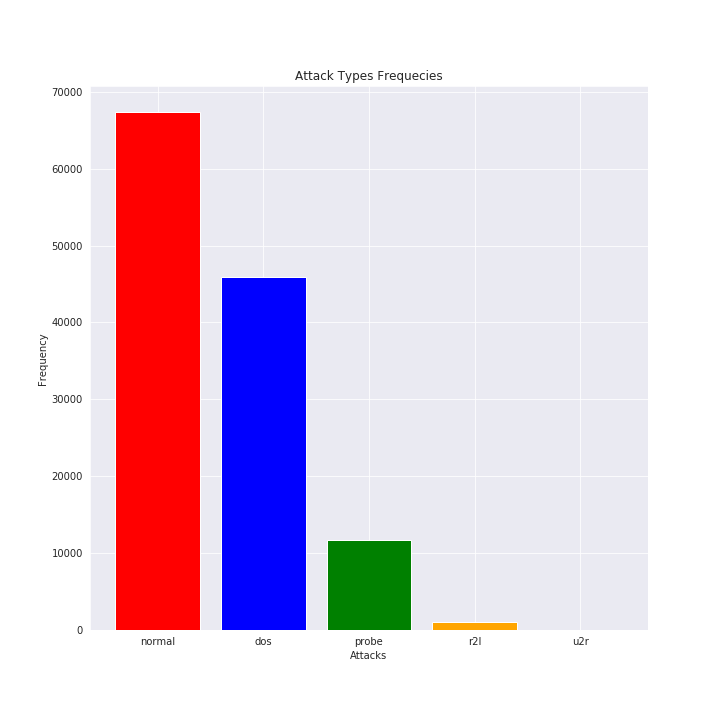
\includegraphics[scale=0.5]{figures/attack_types_frequencies.png}
\caption{The bar graph represents the frequency of different types of attacks. The graph shows that "normal" has the highest frequency, indicating that there were no attacks or suspicious activities during that period. The "dos" attack has the second-highest frequency, while the "probe" attack has the third-highest frequency.}
\label{fig:attack_types_frequencies}
\end{figure}


\begin{figure}[htbp]
\centering
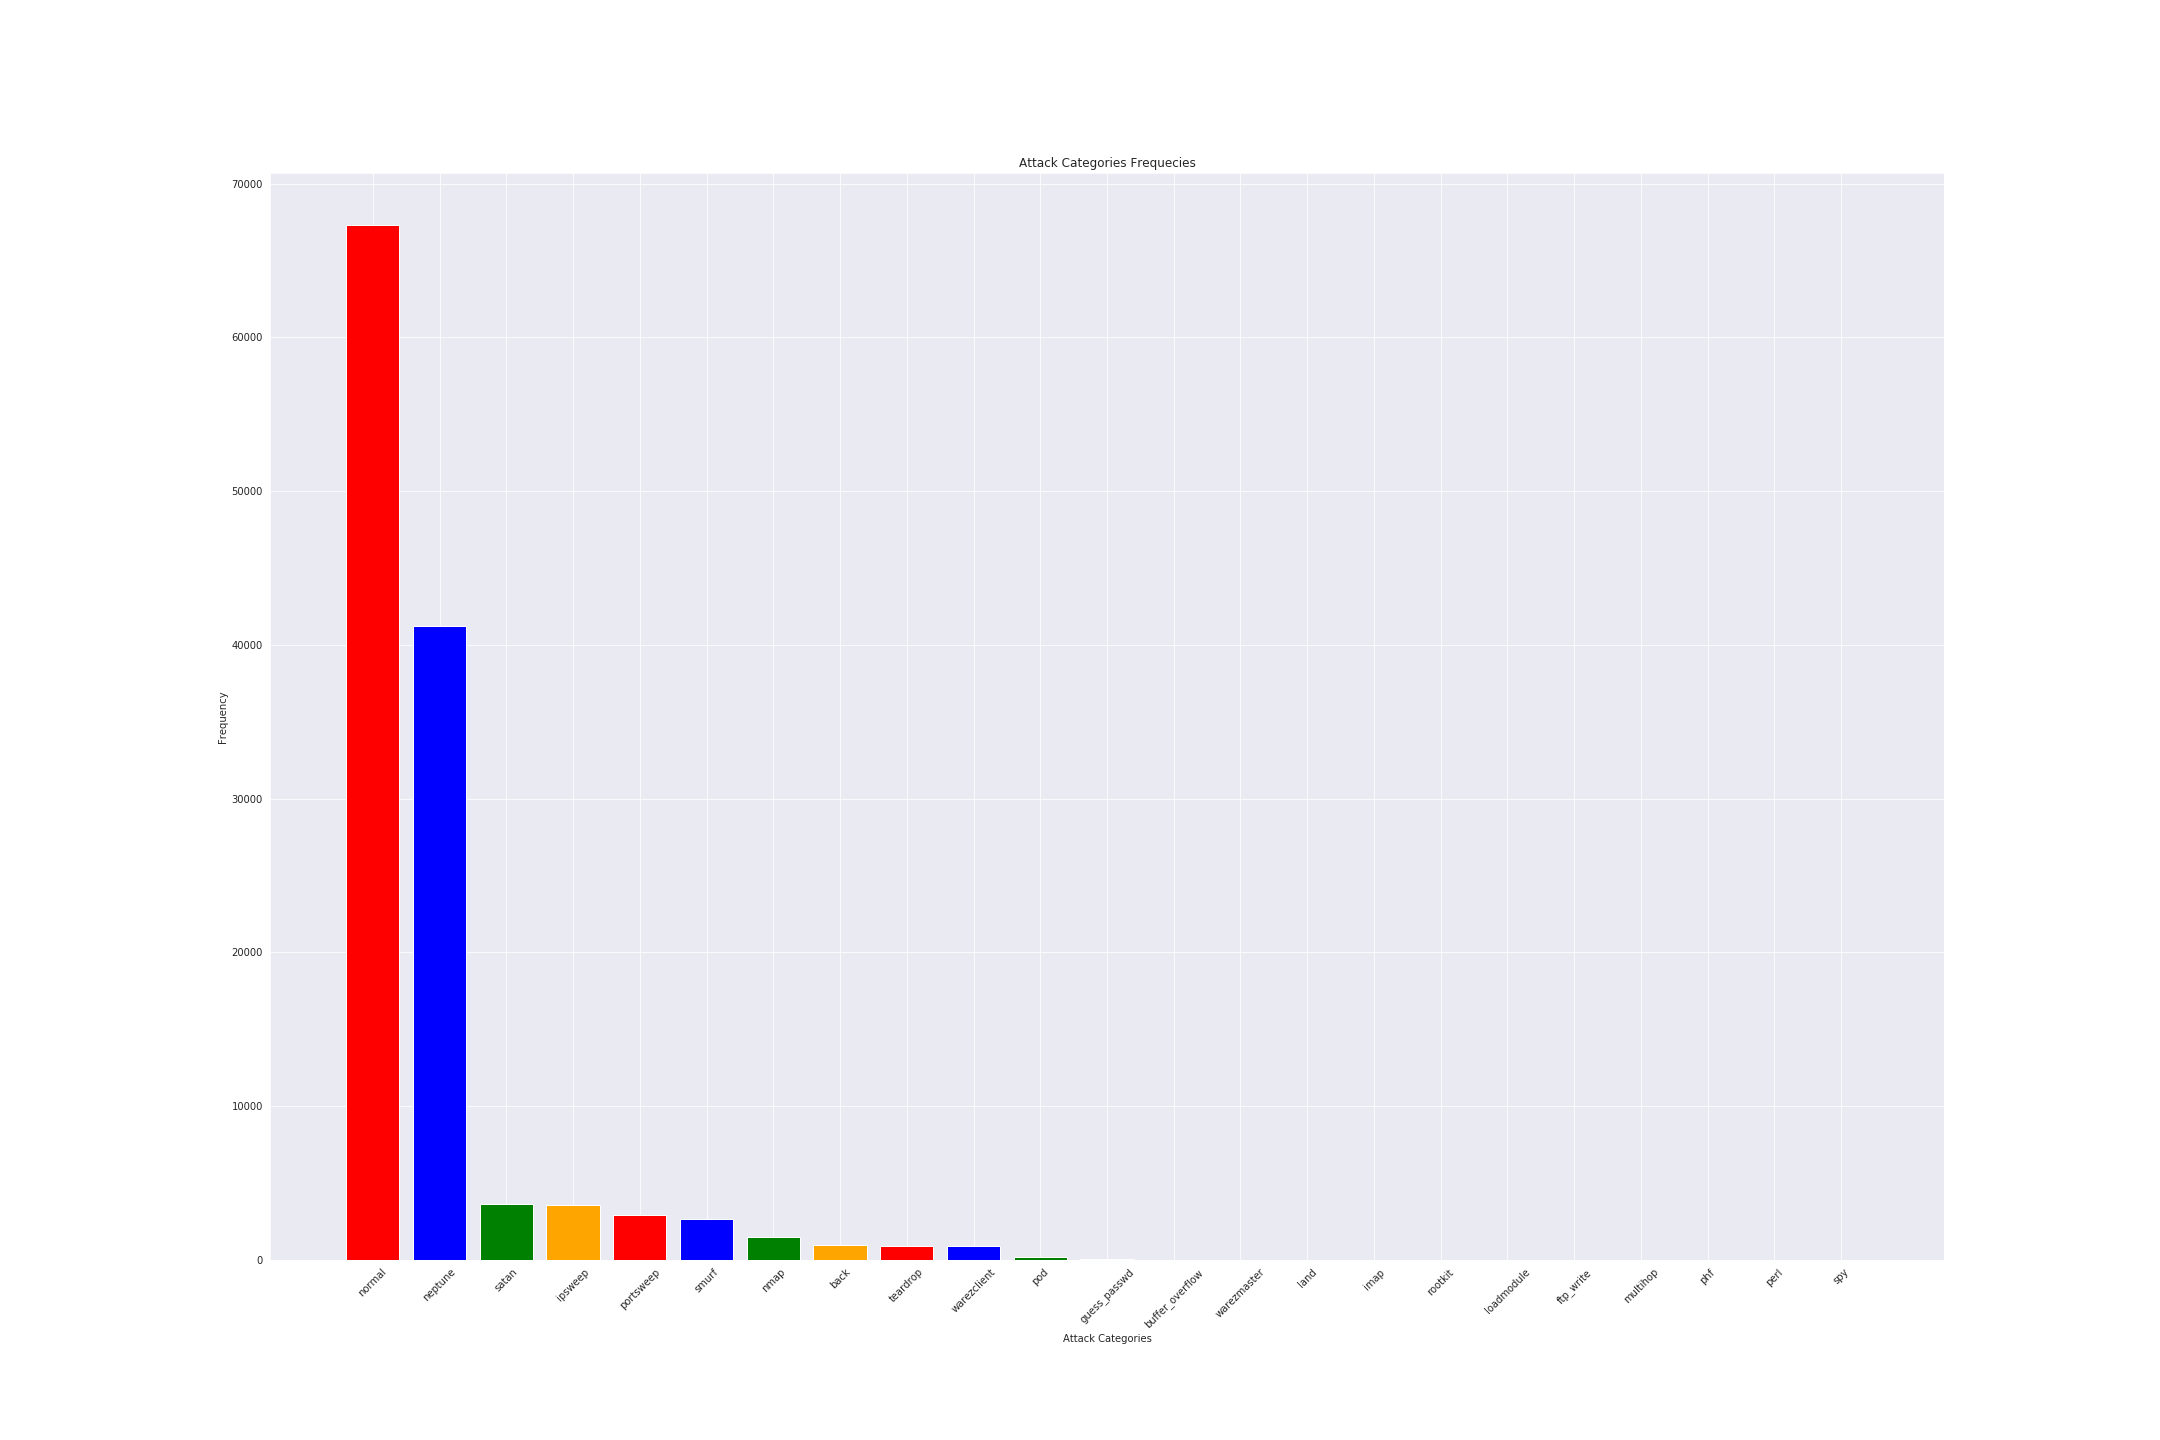
\includegraphics[scale=0.2]{figures/attack_categories_frequencies.png}
\caption{The graph displays the frequency of different attack categories in the dataset. The analysis reveals that the normal attack category has the highest frequency. The second-highest frequency corresponds to the neptune attack, which falls under the dos attack category. The third-highest frequency corresponds to the satan attack, which falls under the probe attack category.}
\label{fig:attack_categories_frequencies}
\end{figure}

\begin{figure}[htbp]
\centering
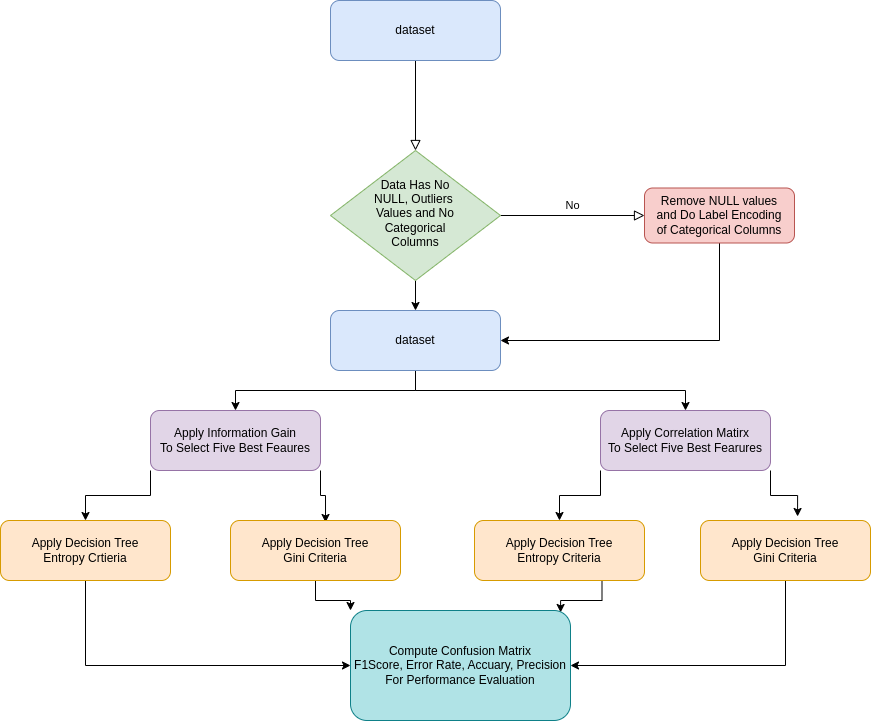
\includegraphics[scale=0.5]{figures/decision_tree.drawio.png}
\caption{flowchart decision tree pipeline}
\label{fig:dt_pipeline}
\end{figure}



\begin{figure}[htbp]
\centering
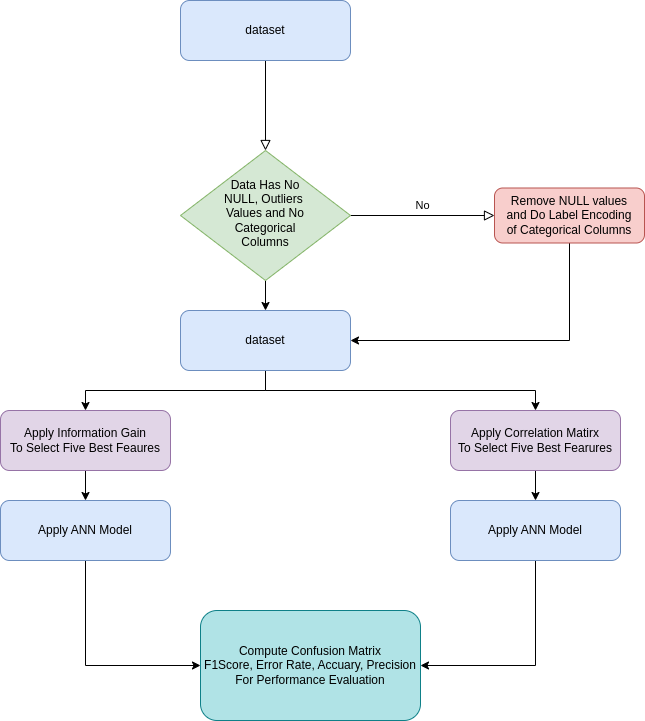
\includegraphics[scale=0.5]{figures/Ann_model.png}
\caption{flowchart ANN pipeline}
\label{fig:ANN_pipeline}
\end{figure}



\begin{figure}[htbp]
\centering
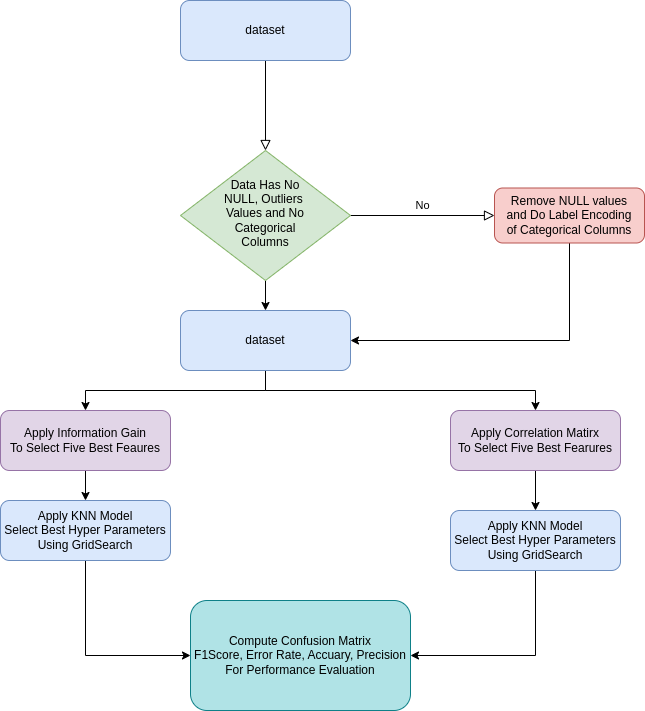
\includegraphics[scale=0.5]{figures/KNN.png}
\caption{flowchart KNN pipeline}
\label{fig:KNN_pipeline}
\end{figure}

\begin{figure}[htbp]
\centering
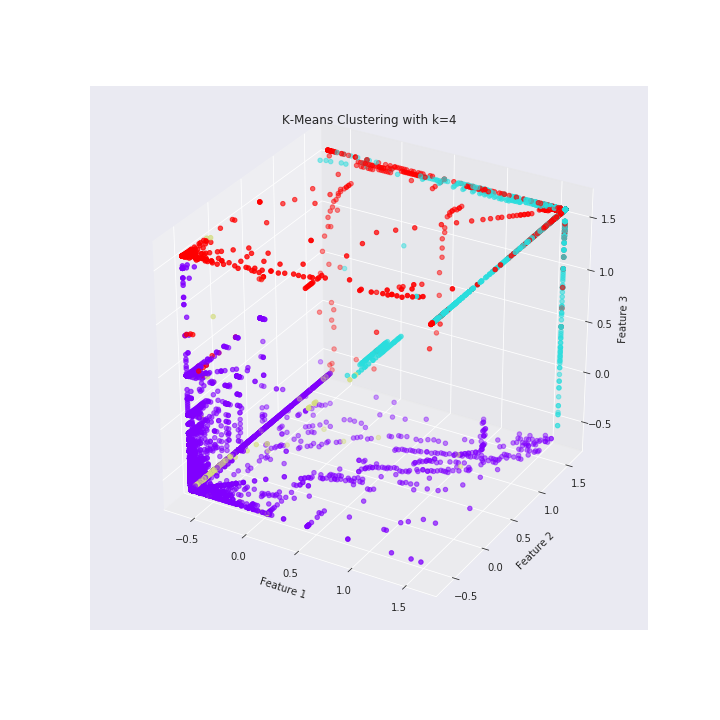
\includegraphics[scale=0.5]{figures/kmeans_cluster.png}
\caption{Scatters Plot K-Means Clusters Selected Based on Features Selected using Correlation Matrix}
\label{fig:IG_Cluters}
\end{figure}

\begin{figure}[htbp]
\centering
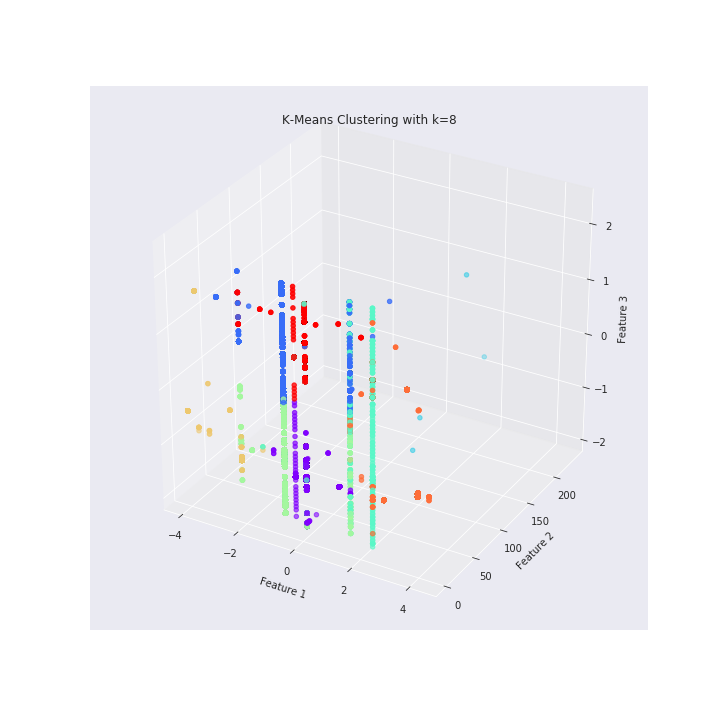
\includegraphics[scale=0.5]{figures/kmeans_cluster_1.png}
\caption{Scatters Plot K-Means Clusters Selected Based on Features Selected using Information Gain}
\label{fig:Corr_Clusters}
\end{figure}

\begin{figure}[htbp]
\centering
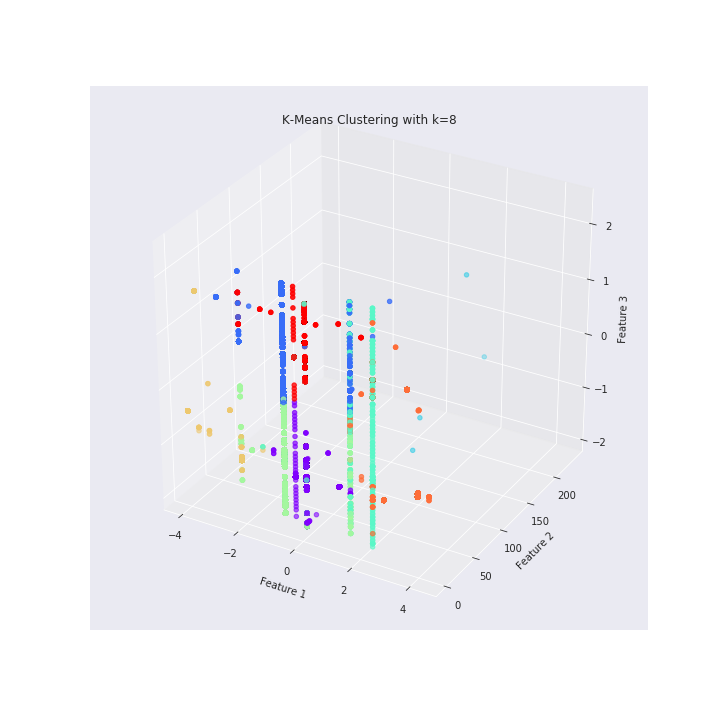
\includegraphics[scale=0.5]{figures/kmeans_cluster_1.png}
\caption{Scatters Plot K-Means Clusters Selected Based on Features Selected using PCA}
\label{fig:PCA_Cluters}
\end{figure}

\begin{figure}[htbp]
\centering
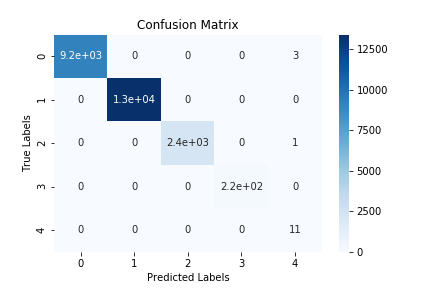
\includegraphics[scale=0.5]{figures/cm_dt_ig_entropy.png}
\caption{Confusion Matrix Decision Tree Entropy Criteria Features Selected Using Information Gain}
\label{fig:dt_cm_entrop_ig}
\end{figure}


\begin{figure}[htbp]
\centering
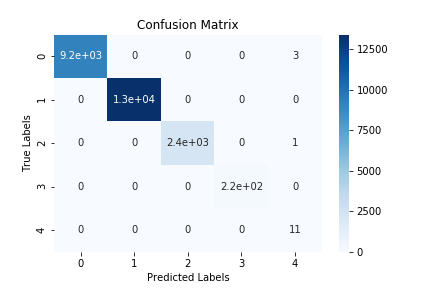
\includegraphics[scale=0.5]{figures/cm_dt_ig_gini.png}
\caption{Confusion Matrix Decision Tree Gini Criteria Features Selected Using Information Gain}
\label{fig:dt_cm_gini_ig}
\end{figure}

\begin{figure}[htbp]
\centering
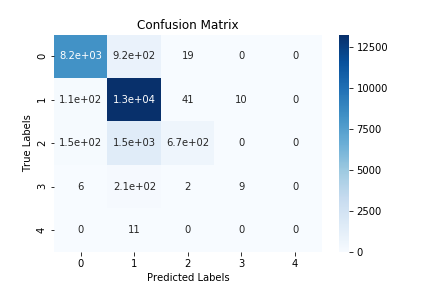
\includegraphics[scale=0.5]{figures/cm_dt_corr_entropy.png}
\caption{Confusion Matrix Decision Tree Entropy Criteria Features Selected Using Correlation matrix}
\label{fig:dt_cm_gini_corr}
\end{figure}

\begin{figure}[htbp]
\centering
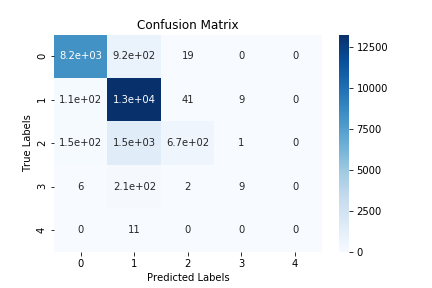
\includegraphics[scale=0.5]{figures/cm_dt_corr_gini.png}
\caption{Confusion Matrix Decision Tree Gini Criteria Features Selected Using Correlation matrix}
\label{fig:dt_cm_gini_corr}
\end{figure}

\begin{figure}[htbp]
\centering
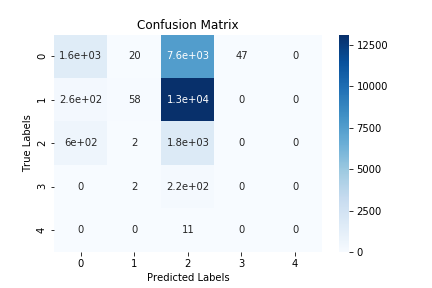
\includegraphics[scale=0.5]{figures/cm_ann_corr.png}
\caption{Confusion Matrix ANN Features Selected Using Correlation matrix}
\label{fig:dt_cm_gini_corr}
\end{figure}


\begin{figure}[htbp]
\centering
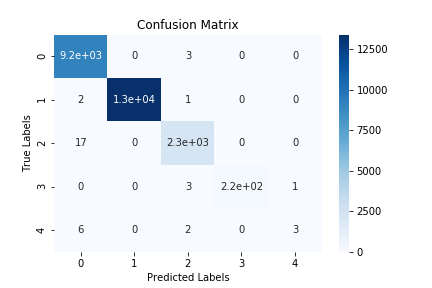
\includegraphics[scale=0.5]{figures/cm_ann_ig.png}
\caption{Confusion Matrix ANN Features Selected Using Correlation matrix}
\label{fig:dt_cm_gini_corr}
\end{figure}

\begin{figure}[htbp]
\centering
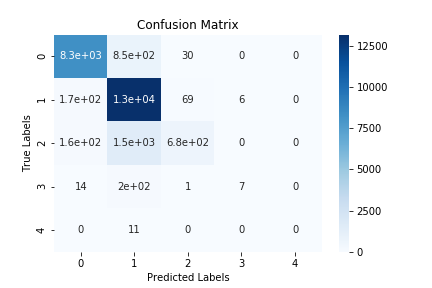
\includegraphics[scale=0.5]{figures/cm_knn_corr.png}
\caption{Confusion Matrix KNN Features Selected Using Correlation matrix}
\label{fig:dt_cm_gini_corr}
\end{figure}

\begin{figure}[htbp]
\centering
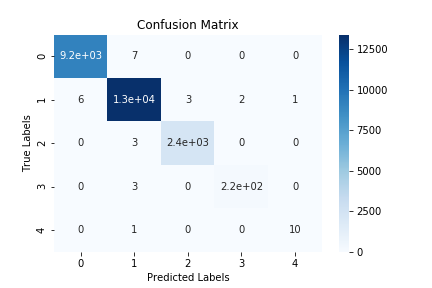
\includegraphics[scale=0.5]{figures/cm_knn_ig.png}
\caption{Confusion Matrix KNN Features Selected Using Information Gain}
\label{fig:dt_cm_gini_corr}
\end{figure}


\end{document}